\documentclass[12pt,a4paper]{article}
\usepackage[utf8]{inputenc}
\usepackage[french]{babel}
\usepackage[T1]{fontenc}
\usepackage{amsmath}
\usepackage{amsfonts}
\usepackage{amssymb}
\usepackage{geometry}
\usepackage[svgnames,dvipsnames]{xcolor}
\usepackage[babel=true]{csquotes}
\usepackage{array}
\usepackage{graphicx}
\usepackage{caption} 
\usepackage{multicol}
\usepackage{mathrsfs}
\usepackage{fancybox}
\usepackage{fancyhdr}
\usepackage{pifont}
\usepackage{manfnt}
\usepackage{dsfont}
\usepackage{hyperref}

\geometry{top=2.5cm, bottom=2.5cm, left=2.5cm, right=2.5cm}
\title{{\Huge \textbf{TP4}} \\ \bigskip {\Huge \textbf{ADM}} \\ \bigskip \bigskip \bigskip VALDEYRON Mathieu \\ \bigskip \bigskip \emph{M1 SSD}}

\begin{document}

\section{Test lisse sur le bloc des deux premiers chiffres significatifs}


L'objectif de cette partie est de reprendre la méthodologie de l'article (A CITER) sur la construction des tests lisses d'adéquation, pour l'appliquer à la loi de Benford sur le bloc des deux premiers chiffres significatifs.

Nous allons ainsi étendre les tests $T_{K}$ utilisés précédemment sur le premier chiffre significatif, pour les appliqués sur le bloc des deux premiers chiffres, et ainsi voir si les conclusions de rejet parmi les pays restent les mêmes.
\\

Dans un premier temps nous construirons donc ces nouveaux tests. Puis dans un second nous observerons leurs courbes de puissance par rapport à deux autres tests : $\chi^{2}$ et Freedman-Watson $(U^{2})$, sur deux alternatives : Rodriguez et Pietronero. Cela s'inspire complètement de (A CITER).


\subsection{Préambule/Cadre Théorique \\}


\textbf{1) Loi de Benford sur le bloc des deux premiers chiffres significatifs :}
\\

Soit $X \in [1;10[$ la mantisse de notre nombre aléatoire. \\
On suppose que $\mathbb{P}(X \leq d) = \log_{10}(d)$ pour tout $d \in [1;10[$. C'est à dire $X$ suit la loi de Benford continue.
\\

Considérons $Y \in [\![ 10; 99 ]\!]$ les deux premiers chiffres significatifs de X. Alors par un raisonnement analogue à la construction de la loi de Benford sur le premier chiffre :
\begin{align*}
\forall y \in [\![ 10; 99 ]\!], \quad \mathbb{P}(Y=y) & = \mathbb{P} \left( \dfrac{y}{10} \leq X < \dfrac{y}{10} + \dfrac{1}{10}\right) \\
& = \log_{10}\left( \dfrac{y}{10} + \dfrac{1}{10} \right) - \log_{10}\left( \dfrac{y}{10} \right) \\
& = \log_{10} \left( \dfrac{y+1}{y} \right) \\
& = \log_{10} \left( 1 + \dfrac{1}{y} \right)
\end{align*}

\textbf{2) Théorèmes (issus de A CITER) :}
\\

Tout repose sur le théorème suivant. Il explique comment construire une famille de tests lisses d'adéquation, indéxée par l'entier $K$. \\

\textbf{Théorème 1)} : Soit $G$ une loi cible, ayant pour densité $f$ par rapport à une mesure dominante $\nu$. Soit $(X_{1}, X_{2}, ..., X_{n})$ un $n$-échantillon issu de $X \sim G_{A}$. On veut tester $H_{0}$ : $G_{A} = G$, contre $H_{1}$ : $G_{A} \ne G$. \\

Soit $\{ h_{0} \equiv 1, h_{k}, k \geq 1 \}$ une famille de fonctions orthonormales par rapport à $f$, c'est à dire $\displaystyle \int h_{k}(x)h_{k^{'}}(x)f(x) \, \mathrm{d \nu}(x) = \delta_{kk^{'}}$, la fonction delta de Kronecker. \\
Soit $U_{k} = n^{-1/2} \sum \limits_{i=1}^{n} h_{k}(X_{i}) $, et soit pour un entier $K \geq1$, $T_{K} = \sum \limits_{k=1}^{K} U_{k}^{2}$. \\ 
Alors sous $H_{0}$, $T_{K} \xrightarrow[n \to +\infty]{\mathcal{L}} \chi_{K}^{2}$ , et un test de niveau asymptotique $\alpha$ rejette $H_{0}$ au profit de $H_{1}$ si la valeur observée de $T_{K}$ dépasse $x_{1- \alpha}$ le quantile d'ordre $1- \alpha$ d'une loi $\chi_{K}^{2}$. \\

Nous allons maintenant spécialisé ce théorème au cas où $G$ est la loi de Benford précédente sur le bloc des deux premiers chiffres significatifs. Nous obtiendrons ainsi plusieurs tests d'adéquation $T_{K}$ pour $G$. \\
Pour ce faire il nous faut calculer des fonctions orthonormales $h_{k}$ associées à $G$ comme dans le théorème ci-dessus. Nous utilisons le résultat suivant (qui est général) : \\

\textbf{Théorème 2)} : Soit $X \sim G$, et $\mu_{k} = \mathbb{E}(X^{k})$, pour $k \geq0$. Soit aussi la matrice $M_{k} = [\mu_{i+j}]_{i,j=0,...,k-1}$, le vecteur $\lambda_{k} = (\mu_{k}, \mu_{k+1}, ..., \mu_{2k-1})^{T}$, et la constante $c_{k} = \mu_{2k} - \lambda_{k}^{T} M_{k}^{-1} \lambda_{k}$. Alors les polynômes :
\begin{center}
$h_{k}(x) = c_{k}^{-1/2} ( x^{k} - (1,x,x^{2},...,x^{k-1}) M_{k}^{-1} \lambda_{k} )$
\end{center}
satisfonts le théorème précédent. \\

Heureusement pour nous, la loi de Benford à deux chiffres est bornée p.s., et donc admet un moment pour tous les ordres. Nous avons donc tout les éléments de "la recette de cuisine".


\subsection{Construction des tests lisses $T_{K}$ : \\}


Soit $X$ suivant la loi de Benford sur le bloc des deux premiers chiffres significatifs, $\forall x \in [\![ 10; 99 ]\!], \quad \mathbb{P}(X=x) = \log_{10} \left( 1 + \dfrac{1}{x} \right)$. On note $X \sim LB(2)$. \\

Cette partie de construction a été effectuée sur R, et toute les commandes se trouvent en annexe. \\

Nous commençons par calculer les fonctions orthonormales $h_{k}$ du théorème numéro 2) ci-dessus, associées à la $LB(2)$. On obtient : \\

$h_{1}(x) = -1.54751771 + 0.04010177 x$ \\

$h_{2}(x) = 2.795867953 - 0.167441591 x + 0.001736457 x^2$ \\

$h_{3}(x) = -5.18781 + 4.869054e^{-01} x - 1.155519e^{-02} x^2 + 7.630402e^{-05} x^3$ \\

$h_{4}(x) = 9.725235 - 1.237520 x + 4.769440e^{-02} x^2 - 6.950207e^{-04} x^3 + 3.371880e^{-06} x^4$ \\

Avec ces quatre fonctions nous pouvons donc construire $T_{K}$ pour $1 \leq K \leq 4$. Le choix de $K$ est important : si il est trop grand alors le test sera très peu puissant, et si il est trop petit alors il le sera également sur certaine alternative. \\
Dans le package associé à (A CITER), on peut calculer les tests pour $K$ entre $1$ et $7$. Pour des raisons pratiques ici, nous n'avons pas pu calculer les $h_{k}$ pour $k \geq 5$. En effet la $LB(2)$ a un support entre $10$ et $99$, et ses moments deviennent très rapidement élevé. Or dans le théorème numéro 2), nous calculons l'inverse de $M_{k}$, ce qui en fait une matrice avec de très petit coefficients. Petit à tel point que le logiciel "plante" car il "ne peut pas effectuer de division par zéro" lors du calcul de l'inverse. Autrement dit, R considère $M_{k}$ comme une matrice non-inversible, ce qui n'est pourtant pas le cas. \\
Cependant, cela n'est pas gênant, car comme nous pourrons le voir plus tard lors du calcul des courbes de puissances, le test préféré est celui du $T_{2}$, surpassant $T_{3}$ et $T_{4}$. Ce qui fait des $T_{K}$, $K \geq 5$, de mauvais candidats. \\

Nous pouvons donc maintenant calculer la statistique $T_{K}$ pour $1 \leq K \leq 4$, et effectuer le test proposé dans le théorème numéro 1) : On rejette $H_{0}$ si $T_{K}$ dépasse le quantile d'ordre $1- \alpha$ de sa loi sous $H_{0}$. \\
Pour une observation $T_{K}(\omega)=t$, nous calculons la p.value associé : $\mathbb{P}_{H_{0}}(t \leq T_{K})$. Si $n$, le nombre de $X_{i}$, est grand, alors on peut approximer la p.value asymptotiquement par $\mathbb{P}(t \leq \chi^{2}_{K})$. Dans la pratique, si $n \leq 100$, on fait l'approximation par Monte-Carlo, et sinon on la fait par approximation asymptotique du $\chi^{2}_{K}$. \\

Justification du choix $n > 100$ : \\

Ci-dessous, voici en couleur les fonctions de répartition empirique issues d'échantillons de taille 10 000 de $T_{K}$ (pour $n=101$, et $n=102$ données), et générés sous $H_{0}$. En noir la fonction de répartition théorique d'un $\chi^{2}_{K}$. Un graphique pour chaque $1 \leq K \leq 4$. \\

On constate que pour n > 100, l'ecdf de $T_{K}$ est quasiment égale à la fonction de répartition théorique d'une $\chi^{2}_{K}$. A tel point qu'il est extrêmement difficile de distinguer cette dernière, c'est à dire la courbe noire, et cela même en zoomant (elle existe bien sur chaque graphique !).


\begin{center}
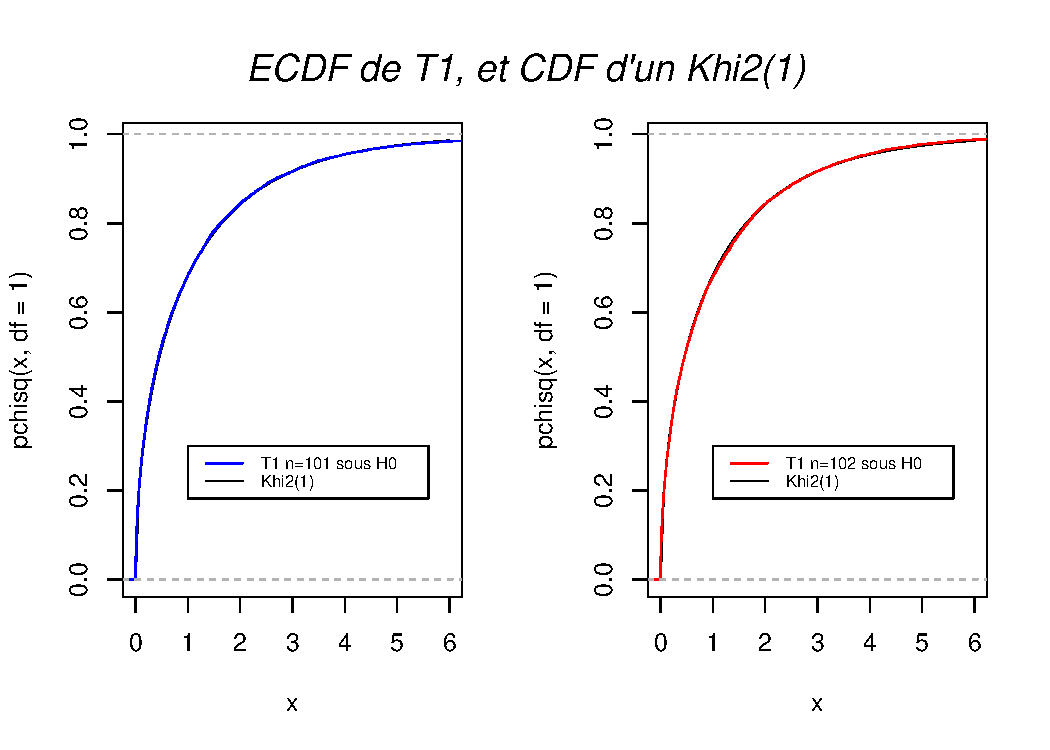
\includegraphics[scale=0.9]{ECDF1.pdf}
\end{center}

\begin{center}
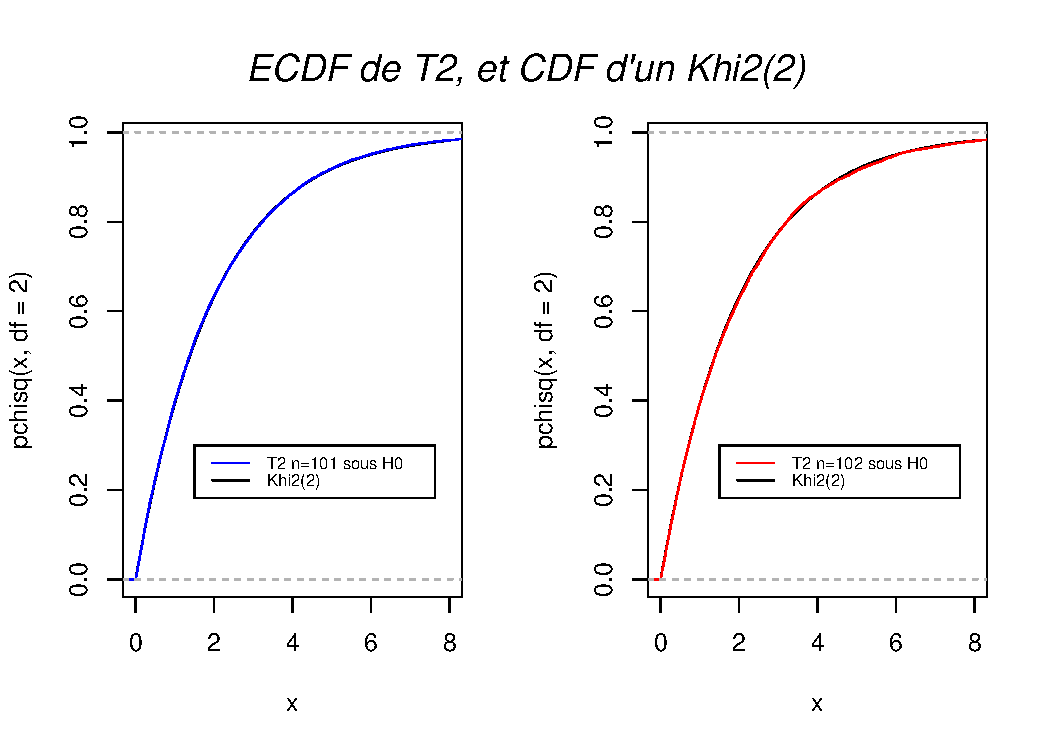
\includegraphics[scale=0.9]{ECDF2.pdf}
\end{center}

\begin{center}
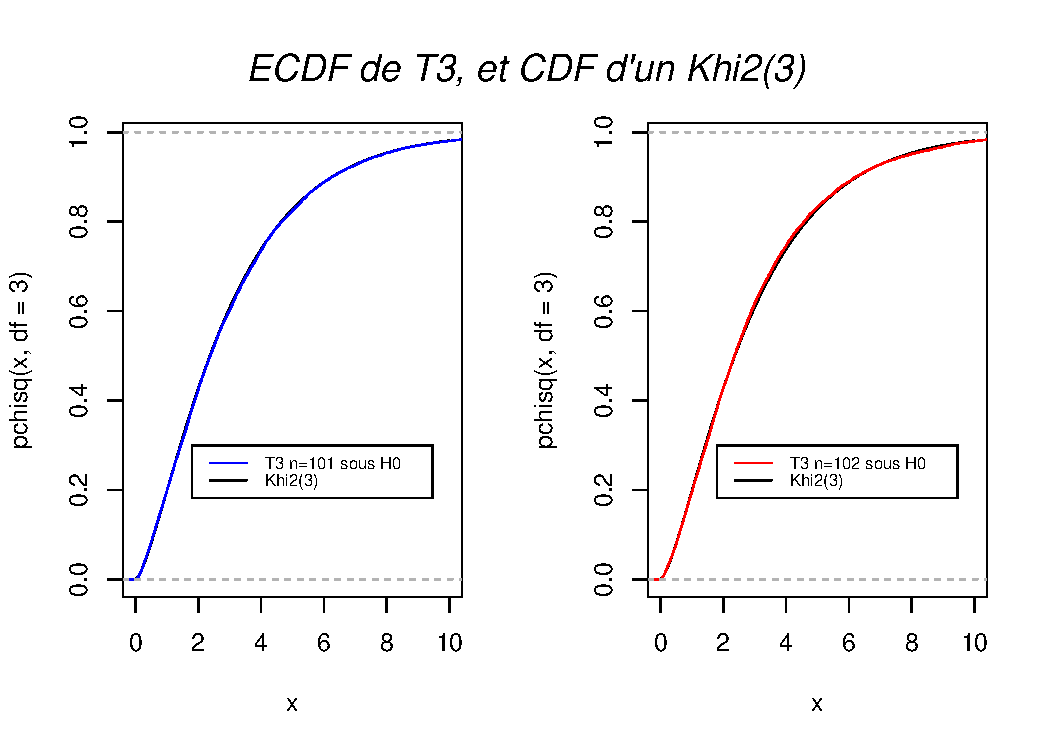
\includegraphics[scale=0.9]{ECDF3.pdf}
\end{center}

\begin{center}
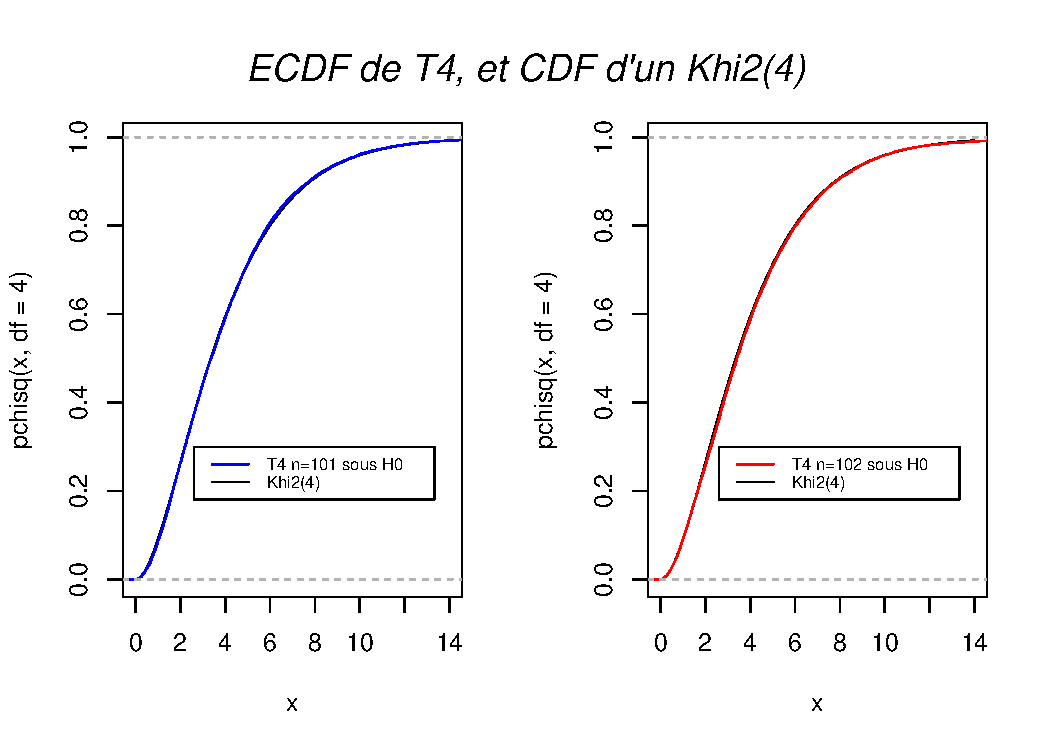
\includegraphics[scale=0.9]{ECDF4.pdf}
\end{center}


Nous avons même recommencé l'opération, toujours avec des échantillons de 10 000 $T_{k}$, mais cette fois-ci pour $n=50$. En bleu la fonction de répartition empirique de $T_{k}$, et en noir la fonction de répartition théorique d'un $\chi_{K}^{2}$. \\

On constate toujours une extrême proximité des courbes bleus et noires. C'est pourquoi le choix de $n > 100$ est même peut-être trop exigeant.


\begin{center}
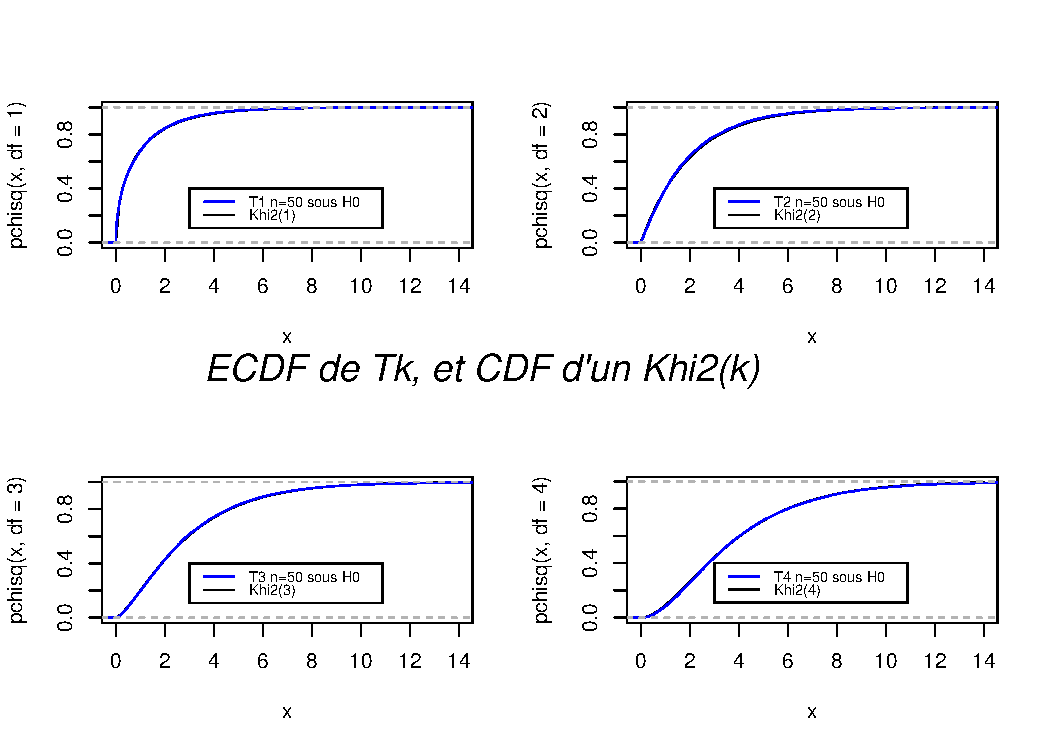
\includegraphics[scale=0.9]{ECDF5.pdf}
\end{center}


\subsection{Comparaison des puissances avec d'autres tests : \\}


Nous allons présenter les courbes de puissance des quatre tests $T_{k}$ construits ci-dessus, du test du $\chi^{2}$, et de celui de Freedman-Watson $(U^{2})$, sur deux alternatives à la $LB(2)$ : La Rodriguez et la Pietronero bivarié. \\
	
$\rightarrow$ Le test du $U^{2}$ étant moins connu que celui du $\chi^{2}$, on rappelle sa statistique : \\

Pour $d \in [\![ 10; 99 ]\!]$, on pose $\hat{p_{d}} = n_{d}/n$ la proportion de $d$ dans l'échantillon $(X_{1}, X_{2}, ...,X_{n})$, et $\pi_{d}$ les probabilités théorique de la $LB(2)$. Soit aussi $S_{d} = \sum \limits_{i=10}^{d} \hat{p_{i}}$ et $S_{d}^{*} = \sum \limits_{i=10}^{d}  \pi_{i}$. Posons $Z_{d} = S_{d} - S_{d}^{*}$ l'écart entre la fonctions de répartitions empirique et la fonction de répartition théorique de la $LB(2)$. Posons également $t_{d} = (\pi_{d} + \pi_{d+1})/2$ pour $d=10,11,...,98$, et $t_{99} = (\pi_{99} + \pi_{10})/2$. Alors :
\begin{center}
$U^{2} = \dfrac{1}{n} \sum \limits_{d=10}^{99} (Z_{d} - \bar{Z})^{2} t_{d}$
\end{center}

$\rightarrow$ On présente également les alternatives à la $LB(2)$ : \\

1) Rodriguez bivarié : ($\gamma =-1$ : on retrouve la $LB(2)$)
\begin{center}
$\mathbb{P}(X=d) = \left\{
    \begin{array}{ll}
    \log_{10} ( 1 + \dfrac{1}{d} ) & \mbox{si } \gamma = -1 \\
    \dfrac{1}{810} \left( 9+19\ln(10)+9d \ln(d) - 9(d+1) \ln(d+1) \right) & \mbox{si } \gamma = 0 \\
    \dfrac{\gamma+1}{90\gamma} - \dfrac{(d+1)^{\gamma+1} - d^{\gamma+1}}{\gamma( 100^{\gamma+1} - 10^{\gamma+1} )} & \mbox{sinon}
    \end{array}
\right.$
\end{center}
\bigskip

2) Pietronero bivarié : ($\gamma =0$ : on retrouve la $LB(2)$)
\begin{center}
$\mathbb{P}(X=d) = \left\{
    \begin{array}{ll}
    \log_{10} ( 1 + \dfrac{1}{y} ) & \mbox{si } \gamma = 0 \\
    \dfrac{d^{-\gamma} - (d+1)^{-\gamma}}{10^{-\gamma} - 100^{-\gamma}} & \mbox{sinon}
    \end{array}
\right.$
\end{center}
\bigskip

Dans (A CITER), voici les courbes de puissances obtenues pour les tests ci-dessus $(T^{2}, \chi^{2}, U^{2})$ portant sur l'adéquation du premier chiffre significatif avec la $LB(1)$ (loi de Benford simple), et pour les alternatives correspondantes univariées :


\begin{center}
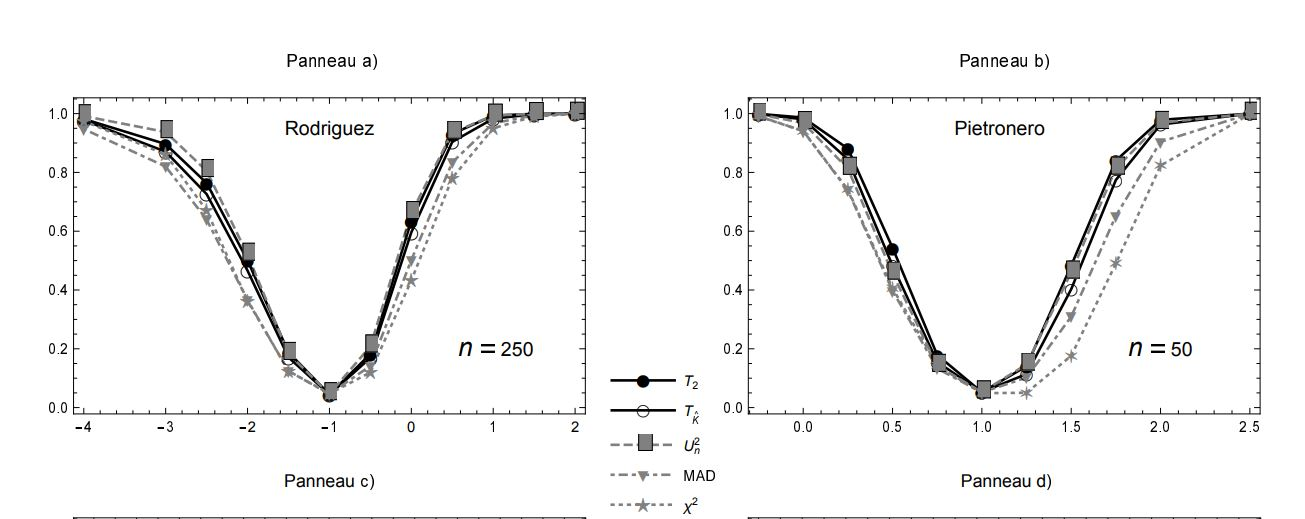
\includegraphics[scale=0.6]{Capture1.JPG}
\end{center}


Les tests du $T^{2}$ et du $U^{2}$ sont très bon. Tandis que celui du $\chi^{2}$ est très mauvais. Voyons voir si nous avons équivalence avec le cas bivarié à deux chiffres significatifs. \\

Nous allons effectuer des simulations pour trois choix de $n$ : 50, 100, et 150. Ces ordres de grandeurs correspondent à la taille moyenne des échantillons que l'on peut rencontrer sur les données covid des pays. \\
Notons également que chaque test sera effectué au niveau $5\%$. \\
Dans un premier temps, pour chaque choix de $n$, nous approximons les quantiles de référence de chacun des tests par les quantiles empiriques d'ordres $95\%$ des statistiques précédentes sous $H_{0}$ : $X \sim LB(2)$. Cela dans le but d'être sûr de bien comparer la puissance de différent tests à $5\%$. Nous effectuons 100 000 réplications pour cela. \\
Ensuite pour chaque alternative, chaque choix de $n$, nous allons générer 10 000 échantillons de taille $n$, pour un $\gamma$ fixé, et appliquer les tests à chacun de ces échantillons, puis compter le nombre de rejet parmi le nombre total afin d'approximer par Monte-Carlo $\mathbb{P}_{\gamma}(\Phi = 1)$. Nous allons parcourir une centaine de $\gamma$ sur un intervalle $[-5;5]$. \\

Notons que nous obtenons une erreur d'approximation des probabilités qui ne dépasse jamais les $0.01$ pour Monte-Carlo (au niveau de confiance $95 \%$). \\
Nous avons les graphiques suivants :


\begin{center}
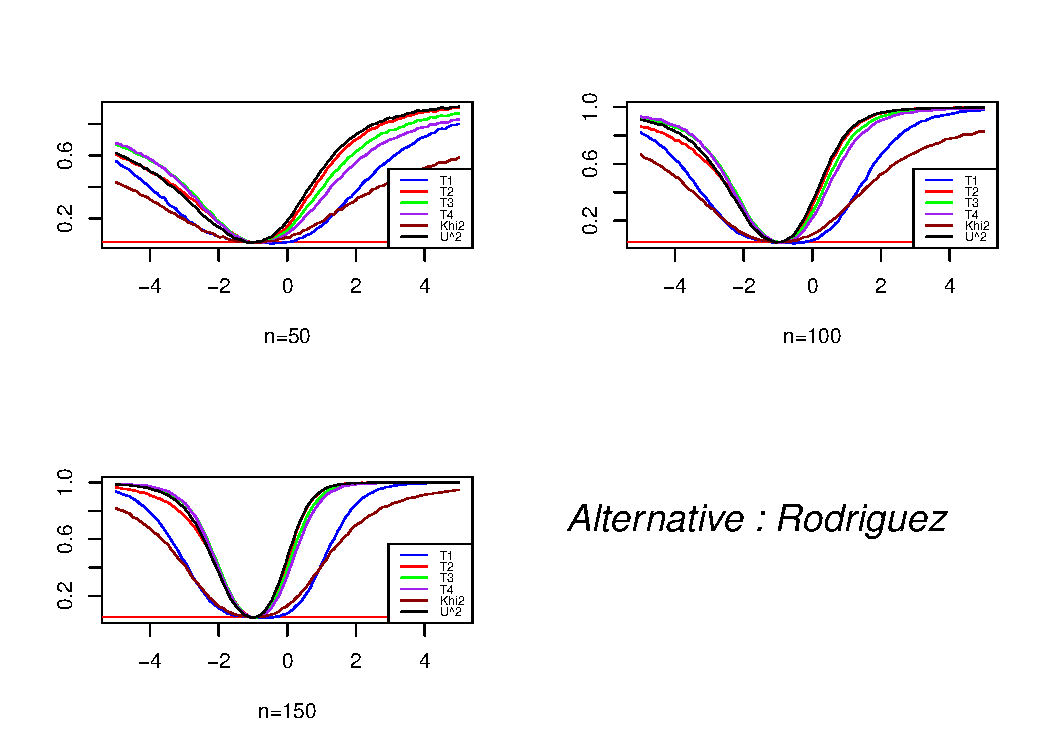
\includegraphics[scale=1]{Rplot1.pdf}
\end{center}
\begin{center}
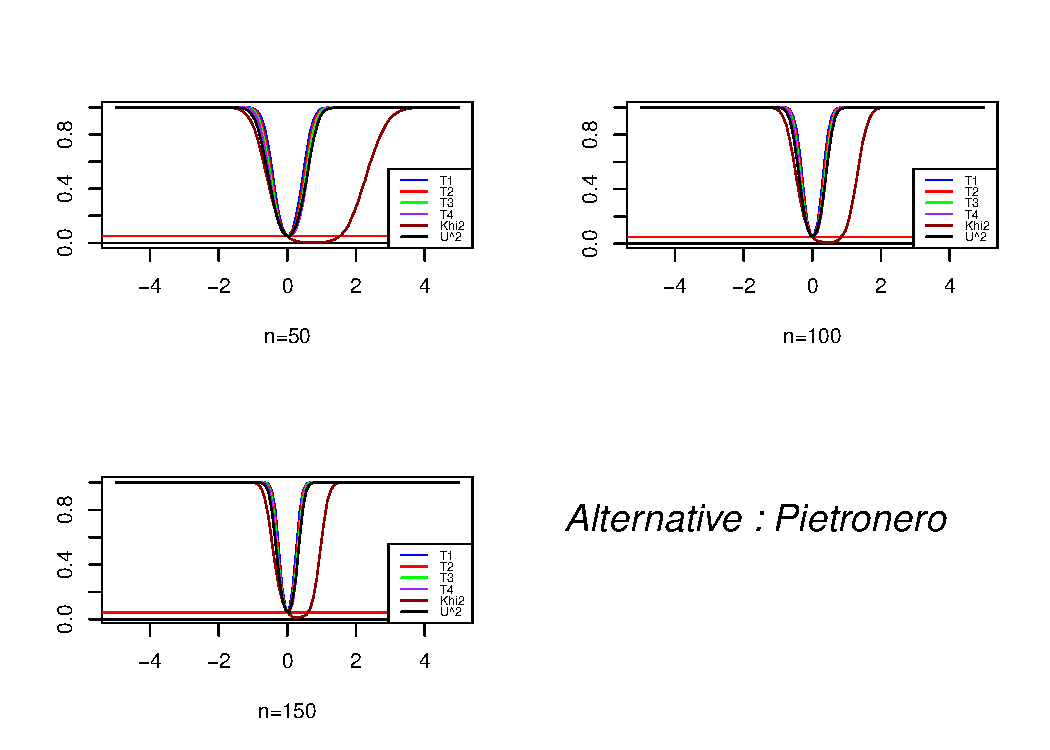
\includegraphics[scale=1]{Rplot2.pdf} 
\end{center}


1) Pour l'alternative Rodriguez tout d'abord. On retrouve le test du $T_{2}$ et celui du $U^{2}$ parmi les meilleurs. Le $U^{2}$ est même légèrement mieux que le $T_{2}$, en particulier pour des $\gamma < -1$. Exactement comme pour le cas univarié. On retrouve aussi un test du $\chi^{2}$ très mauvais. Cependant on constate que les tests $T_{3}$ et $T_{4}$ sont les meilleurs parmi ceux proposés, pour des $\gamma < -1$. On pourra même préférer le $T_{3}$ au $T_{4}$ car pour des $\gamma > -1$, il est meilleur. Par conséquent, si l'on suspecte une alternative Rodriguez avec des $\gamma < -1$ ou bien des $\gamma > -1$, on pourra privilégier le $T_{3}$, ou bien le $U_{2}$. Le problème c'est qu'une telle chose est difficilement suspectable. \\

2) Pour l'alternative Pietronero. Le test du $\chi^{2}$ est toujours très mauvais. Sa courbe vient même toucher $y=0$, pour $x$ entre $0$ et $1$, ce qui est surprenant... Peut-être une erreur lors de la simulation, mais je n'ai pas pu la détecter. Pour les autres tests, le $U^{2}$ est cette fois-ci assez mauvais par rapport aux autres. Comme dans le cas univarié, il est moins bon que le $T_{2}$. Ce dernier $T_{2}$ reste toujours en tête du classement, mais il est dépassé de peu par le test du $T_{1}$. Malheureusement le $T_{1}$ était assez mauvais pour l'alternative Rodriguez. \\

On retrouve tout de même des résultats proches de ceux du cas univarié. On peut même suspecter la même chose pour les alternatives que nous n'avons pas testée, et qui sont présenter dans (A CITER). Dans ces dernières alternatives, le test du $U^{2}$ s'effondrait, et le test du $T_{2}$ restait bon. De plus, juste en considérant les deux alternatives Rodriguez et Pietronero que nous avons présenté, ne sachant pas dans qu'elle situation on se situe dans la pratique, le test du $T_{2}$ est un bon candidat pour les deux alternatives. Nous allons d'ailleurs choisir ce test pour effectuer les analyses des données covid par la suite.







\end{document}